% 1977 年辽宁卷参考题一：有盖圆柱形氨水池，标高 h 与底面半径 r（按源卷第 7 页布局）
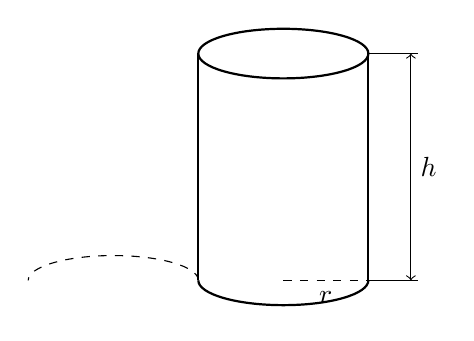
\begin{tikzpicture}[scale=0.9]
  \draw[thick] (1.2,3.2) ellipse (1.2 and 0.35);
  \draw[thick] (0,3.2)--(0,0);
  \draw[thick] (2.4,3.2)--(2.4,0);
  \draw[thick] (0,0) arc[x radius=1.2,y radius=0.35,start angle=180,end angle=360];
  \draw[dashed] (0,0) arc[x radius=1.2,y radius=0.35,start angle=0,end angle=180];
  % 底面半径 r（中心到右缘，虚线）
  \draw[dashed] (1.2,0)--(2.4,0);
  \node[draw=none,below] at (1.8,-0.02) {$r$};
  % 高 h（右侧尺寸线）
  \draw[thin] (2.4,0) -- (3.1,0);
  \draw[thin] (2.4,3.2) -- (3.1,3.2);
  \draw[<->] (3.0,0)--(3.0,3.2) node[midway,right] {$h$};
\end{tikzpicture}
